%% Anonymized manuscript for EAAI double-anonymized review.
%% Author details are in title_page.tex. Do not include this file's
%% author block, CRediT names, or repository URL in the review PDF.

\documentclass[preprint,12pt,authoryear,doubleblind]{elsarticle}

\usepackage{amssymb}
\usepackage{amsmath}
\usepackage{booktabs}
\usepackage{graphicx}
\usepackage{tabularx}
\usepackage{url}
\usepackage{hyperref}

\journal{Engineering Applications of Artificial Intelligence}

\begin{document}

\begin{frontmatter}

\title{Scale-Invariant Baselines Can Certify a Broken Deep Model: Grouped-Normalisation Collapse in Learned Trajectory Screening}

%% Author names and affiliations are supplied only on title_page.tex.

\begin{abstract}
A single feature scaler is often used among a set of data. We show that it can quietly harm a sequence model without warning the practitioner about any problems, even when they apply all the checks they should. A Transformer trained with a scaler averaged over a target group ceases to react to the input on Venus (3.11e-05 prediction standard deviation on unseen missions, 0.6037 validation area under the ROC curve (AUC)). Let's train a gradient boosted tree on the same arrays and nothing is amiss. Its AUC varies by at most 0.0002 across all three normalisation settings, and it finds the task almost perfectly separable while the network cannot separate it at all. Trees here are not affected by the thing that is destroying the network. Severe, but not everywhere - 1 of 4 targets collapses; the remaining ones lose between 0.0003 and 0.0925 AUC while they keep working. The compression is the same across the 5 seeds, and the collapse occurs on 4 of them, it is not due to one unlucky initialisation but is inherent in the preprocessing itself. Our AI contribution is a controlled test of when pooled normalisation breaks a sequence model (survivable across timesteps, not across groups), a check on prediction spread that catches it, and a second failure where the model cannot find a rare class that a tree finds in the same input. The engineering application is screening simulated spacecraft trajectories to save compute.
\end{abstract}

%% Graphical abstract: optional, not supplied. If one is made, upload it as a
%% separate file (531 x 1328 pixels, height by width, or proportionally more).
%% Highlights: submitted as the separate file highlights.docx, as the journal asks.

\begin{keyword}
feature normalisation \sep shortcut learning \sep model diagnostics \sep simulation screening \sep trajectory analysis \sep negative results
\end{keyword}

\end{frontmatter}

\section{Introduction}
\label{sec:intro}

In Monte Carlo trajectory campaigns, the majority of the compute is used on runs that were already sure to fail when they left the parking orbit. These campaigns are a regular occurrence at flight facilities, such as the large dispersion campaign that TESS used to set its trajectory design \citep{nickel2016}. Not only is this expensive, a body of work has been developed to make each propagation even less expensive \citep{massari2017,jia2022}. Another, and obvious, approach is to steer clear of these runs: track the first part of a trajectory and cancel out the ones that will fail. It's a screen we have made. It revealed two failures that we believe are much more than astrodynamics related, and one bad result regarding the screen.

This paper will deal with the first failure. Grouped data was used for training the model and a single feature scaler was fitted for the entire group. It ended up emitting a single constant per group. It's not the surprising part that it happened. What's most interesting is the length of time it took to be noticed. With a mixed validation set it looked fine, since a model can score well if it differentiates groups but cannot differentiate anything within the groups, and validation AUC remained high. A baseline run was executed with a gradient boosted model, with almost perfect results, because the trees divide on the actual values and the scaling on which the network depends is not important to them. Both of the tests we would have used would have told us that the pipeline was healthy.

This isn't, of course, comfortable, as running a simple baseline is good advice. It is common practice for tabular and physical data to be checked by tree ensembles and they are typically the correct choice \citep{chen2016,grinsztajn2022,shwartz2022}. In fact, the very property that makes them good checks in general (invariance to the scale of the features) is the one that makes them insensitive to this specific defect. The check cannot fail the model, so it passes it.

We make three contributions. It is first a controlled decomposition of the collapse, which distinguishes pooling over time from pooling across groups, and shows only the latter to be deadly. Second, a demonstration that a scale-invariant baseline actually approves of the broken configuration, as well as an inexpensive diagnostic that does notice it. Third, another failure of the same kind: the model has no access to a rare class that can be recovered from its own input. We also report something that limits how much the first two matter in practice, which is that the application that inspired them doesn't need a sequence model at all.

This paper is based on scripts in the attached repository that generate all the numbers, which are written to machine-readable artefacts. Those artefacts are then used to create the paper containing tables and figures.

\section{Related Work}
\label{sec:related}

Normalisation is crucial for training deep networks, and there are standard layers (batch, layer, group, instance) that solve a version of the problem \citep{ioffe2015,ba2016,wu2018,ulyanov2016,huang2023}. It has been long known that the ability of a network to train, and not merely the rate at which it trains, depends on the scaling of the inputs \citep{sola1997}. These layers also make some assumptions about the input that they're given. They assume that the feature statistics are stationary, or that they're comparable within each pooling axis. When more than one set of data is measured on the same scaler, but the range of the data is very different, that assumption is already broken before the first layer runs. What we add is a controlled decomposition that shows us that it is not the pooling in general that does the damage, but only the pooling across the groups, and then an observation that the resulting model is not a weak model, but a constant model.

When a shortcut is there, a network will easily learn the easy signals and take the shortcut over the intended structure \citep{geirhos2020,shah2020}. Previous research on Clever-Hans behaviour demonstrates that the models achieve good scores for reasons that are not related to the task \citep{lapuschkin2019}. If the scales are grouped and are not homogenous, there is an exceptionally clean shortcut, the distance between the group centroids. This type of model simply memorizes the difference, and has validation AUC of $>$0.95 but performs no better inside individual groups. That's what we saw. Here, our contribution is a diagnostic (spread of the predictions within a group) which does not need any label and is quite different from the common underfitting. It is also not a modelling problem, but a pipeline level problem, like many which can be found in the shared preprocessing code that no single model owns \citep{chaudhary2018}.

Tree ensembles perform well on tabular and physical data, and often perform with the same or better results than deep models \citep{chen2016,grinsztajn2022,shwartz2022,ke2017,pasaribu2024}, and most practitioners turn to a tree as a baseline for that reason. Their splits are axis-aligned and threshold-based, with a monotone rescaling of a feature having no effect on the splits. It's typically a good thing that it's invariant. It also makes them unable to identify a deadly error in the preprocessing, an error that results in a failure of the network.

The standard ways to overcome a serious imbalance are reweighting, focal loss or resampling \citep{buda2018,lin2017,cui2019}, and the effect of imbalance on the actual learning of a deep classifier is explored in great detail \citep{dong2025}. The two model families have different reactions to it, which is a reason why it is worthwhile to make a comparison at all \citep{wu2021}. In Section~\ref{sec:rare} we report a case in which none of that is the issue: oversampling a rare failure mode by a factor of 19.2 doesn't move its recall at all, but a tree on the same window separates it almost perfectly. It's the same with the evidence in the space domain. The ESA anomaly benchmark shows that current sequence models still struggle with the rare but important events in real satellite telemetry \citep{kotowski2024}, and rare anomaly detection there is still active enough to need uncertainty-aware methods \citep{sadr2022}. This is a type of data that carefully designed LSTM pipelines are able to perform well on when the data is correctly processed in all channels \citep{hundman2018}. It's not the model class, it's the engineering that makes the difference.

Networks have been successfully applied in astrodynamics for trajectory optimization, approximation of optimal control \citep{izzo2019survey,izzo2024,sanchez2018}, cost estimation without complete propagation \citep{li2020deep,izzo2019ml} and learning of a robust low thrust policy with certification via Monte Carlo \citep{zavoli2021}. Learned models also correct orbit predictions from sparse tracking \citep{li2020orbit}, stand in for Monte Carlo when propagating orbit uncertainty forward \citep{zhou2024}, and are used for anomaly and fault detection in spacecraft telemetry \citep{ibrahim2019,naik2020}, where the same family of attention architectures is used as here \citep{jiang2023}. Screening specifically, by means of a learned model selecting which of a very large number of candidate cases get full analysis, is already recognized: an ESA competition on real conjunction data \citep{uriot2020,acciarini2021}, and a benchmark of deep approaches against the classical filters they would replace \citep{stevenson2023}. The final one is the most similar setting, a screening task on a deterministic astrodynamics simulator, measured against non-deep baselines. We could not find an article in this literature that considers early termination of individual Monte Carlo trajectory runs as we do in Section~\ref{sec:screen}. The closest work decreases the cost of each propagation rather than deciding which propagations to start \citep{massari2017,jia2022}. The general idea is to use a learned surrogate instead of part of an expensive simulation \citep{yin2022}.

\section{Setup}
\label{sec:setup}

In total, we developed 70,000 missions that leave the Earth, 10,000 missions to each of seven interplanetary targets (Mercury, Venus, Mars, Jupiter, Saturn, Uranus and Neptune), using NASA's General Mission Analysis Tool. It has an extensively verified two and three body propagator \citep{hughes2014}, and is deterministic. Each mission has six injection offsets, which are the components of the trans orbit insertion burn (\texttt{dv\_V}, \texttt{dv\_N}, \texttt{dv\_B}), and the RAAN, AOP and INC of the parking orbit from which the mission departs. Each is classified as success or failure, and failed ones are further sub-categorised as surface impact, orbit too high, missed target and a few others.

The interplanetary transfers are sampled at a fixed rate of 54,000 s (15 hours) and downsampled to about 100 steps for each mission. This is so that the sequences produced by targets with flight times that vary by 2 orders of magnitude are comparable. Thirteen features are recorded for each step, and include position in the synodic frame, specific orbital energy, flight path angle, normalised target distance and eccentricity. An eighth target was created (the Moon), and is intentionally left out of the study. It is a 6 day transfer inside Earth's neighbourhood, sampled at 60 s, and it doesn't have a cost structure similar to Section~\ref{sec:screen}, or a heliocentric dynamical regime.

The screening task is to observe the first 40\% of the mission's flight path and decide whether or not to abort. Splits are mission based 70/15/15, deterministic in (n, seed). The experiments are all based on a single definition in the repository, so no model is ever scored using data that was used for model selection. It is not a theoretical question. Two of the previous analyses in this project shuffled the same number of missions using the same seed, and in those analyses the same set of missions ended up in both `test' sets.

The sequence model is a Pre-LN Transformer encoder, \texttt{d\_model} 128, 8 heads, 4 layers and CLS token pooling, and 2 heads are connected to a single trunk (one for mission outcome and one for failure mode). It is trained on random length prefixes, so that its predictions are not only at the 40\% mark in the stream but at any point in the stream. The baseline is XGBoost, 300 trees at depth 5, fitted to the same normalised prefix, flattened. It is important to note that the baseline is not working from a feature set derived separately, but from the same view the network sees, which is what `the same input' means throughout this paper. That detail carries most of the argument and we're very rigid with it.

The three conditions are the following sets of normalisations, which only vary in how the feature statistics are combined. All use the same architecture, seed, split, optimiser and epoch budget.

per timestep: every one takes its statistics from the distribution of features at that timestep index, over the missions of one target (Fig.~\ref{fig:modes}). This is the configuration the working system uses.

global: one RobustScaler (median and IQR) per target, pooled across that target's own timesteps.

grouped: one RobustScaler pooled across all timesteps of all targets in a regime group (inner: Mercury, Venus, Mars; outer: Jupiter, Saturn, Uranus, Neptune). This is the setting that was not successful in production.

The third setting isn't a straw man, and here's why. You get a single RobustScaler from nearly all the standard pipeline tutorials, applied to a concatenated training set. No warning is issued and it looks like a normalised array.

\begin{figure}[t]
\centering
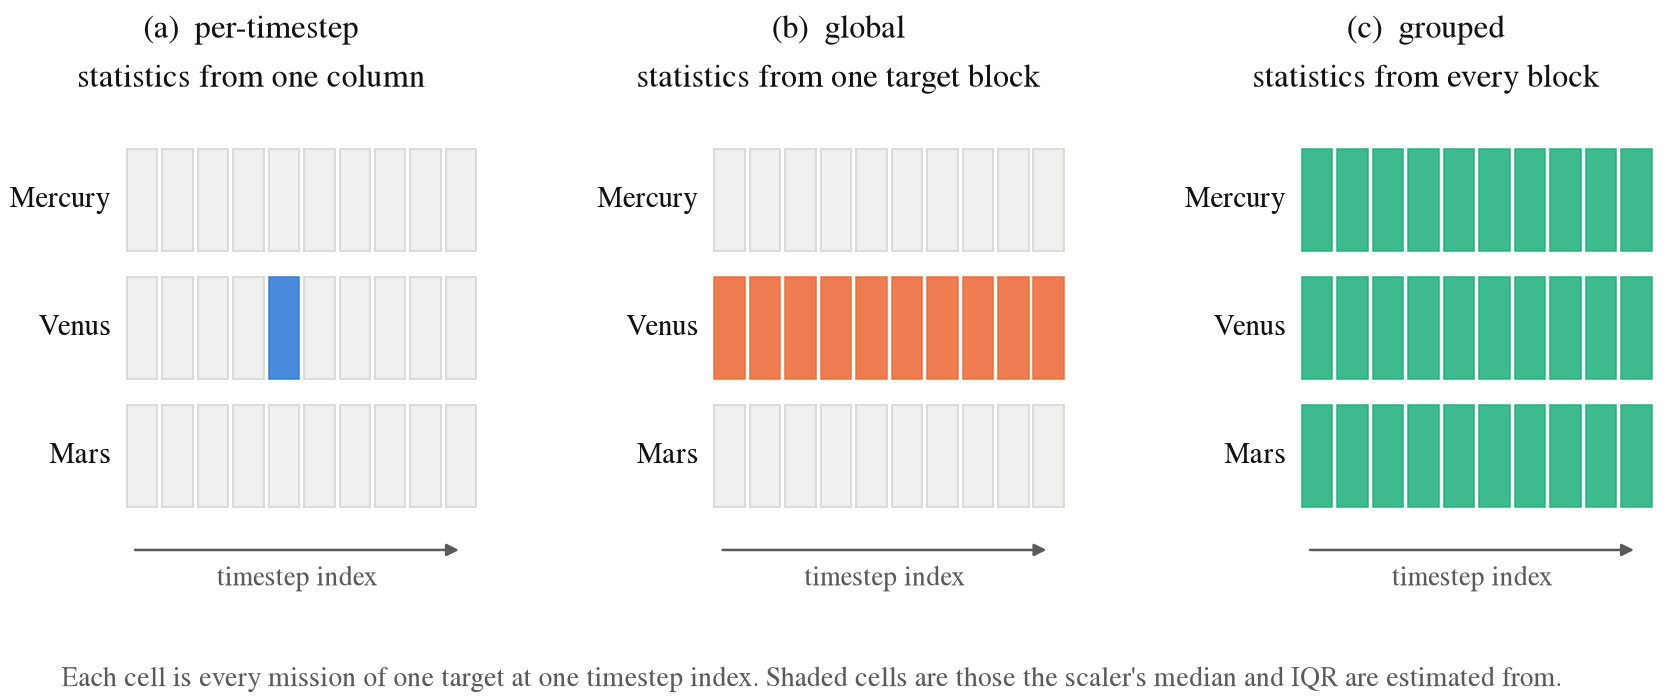
\includegraphics[width=\linewidth]{fig1.png}
\caption{The three normalisation modes, and the only difference between them: from what part of the data does the scaler get its median and IQR? Everything else in training is the same. Each cell is all the missions of one target at one timestep index, and the shaded cells are the ones the median and IQR are estimated from.}
\label{fig:modes}
\end{figure}

\section{Grouped-Normalisation Collapse}
\label{sec:collapse}

A mission's features sweep a wide range as they fly, and the range other targets occupy varies by orders of magnitude. A scaler applied to a set of pooled data will then scale the data on the scale of the largest source of variation in the set. What the screen should be able to tell apart is neither of those things. It is the spread between missions at a particular point in the flight, which by comparison is small. Pooling divides that spread by an arbitrary denominator, which drives the level of the useful signal towards zero and has no effect on the structure between groups. The network is then tasked with learning a difference that is close to the limit of what gradient descent can detect, and Pre-LN layer normalisation filters out a lot of it.

This is used as the signal ratio, defined as the average of the standard deviation of the normalised features across missions, calculated only in the observed window. It's not a limitation you would expect but it does matter. The metric is totally useless averaged over the entire flight, because late timesteps have a huge spread across missions, as the missions that fail have physically diverged by that time, and that spread swamps the early signal so that all conditions appear healthy. The model commits at 40\%, so what's important is the range within the prefix the model observes.

The first result is the decomposition that is controlled. The network is able to operate with the signal being reduced by up to a factor of 23 by pooling across time in a single target. It works on all 4 targets, with a loss of a few thousandths of AUC at most. Another kettle of fish is the pooling of a group. On Venus, the output standard deviation is 3.11e-05, which is one number for every mission, and the AUC drops from 0.9999 to 0.6037.

The term `collapse' is used instead of `underfitting' because of Fig.~\ref{fig:venus}. A low AUC on its own doesn't mean much, because that is what you would get if the model learned something poor or wrong. A distribution on unseen missions that is three ten-thousandths wide is not ambiguous at all. The network is no longer under the control of its input.

The second result is that the collapse is selective, and we report that alongside the case that breaks. In the remaining 3 targets the same manipulation leaves the output still varying, and costs between 0.0003 and 0.0925 AUC. The signal ratio is not a measure of severity either. Jupiter compresses its signal to 0.0247, whereas Mercury compresses its signal to 0.0484, and yet Jupiter loses 0.0003 AUC whilst Mercury loses 0.0925 AUC. This is because Jupiter's task is nicely split up so that even a very weak signal is sufficient. Compression is necessary for the collapse but not sufficient; how hard the underlying task is modulates it. We are not claiming that these data support a rule of the form `it collapses when the ratio is below X'. The counter example is visible in Fig.~\ref{fig:signal}.

One note on scope. This ablation isolates normalisation and no other component of the model, so only the statistics are pooled, with one model trained for each target. The production failure also shared a single trunk across the group, which compounds the problem, since one trunk then has to serve targets whose inputs have all been flattened in the same direction, towards a constant. These numbers therefore represent a minimum damage level of the configuration. They show that pooled normalisation is sufficient on its own to destroy a target, and not that this is a complete reconstruction of the original incident.

Under the grouped setting the tree reports AUC 1.0000 on Venus, the target where the network has collapsed to a constant at AUC 0.6037. Tree AUC changes by at most 0.0002 across settings on all targets, which implies that the choice is not really visible to the tree. Now if one runs it and checks whether or not the features have signal, doing the right and proper thing, he will get an unambiguous yes, and reasonably assume that the deep model needs tuning, and not that the pipeline is broken.

This is the methodological part and it's crucial to pay attention to the exact claim. The information is there and a tree can use it. The baseline is not informative on the question that has to be answered, which is `can the network use it?'. Invariance to feature scaling is typically a good reason to reach for a tree as a diagnostic, and is precisely why it is blind here. The check is orthogonal to the defect by construction, so no matter how carefully one works the check could not have helped.

Accuracy on a mixed validation set does not catch the collapse, because a per group constant ranks the groups correctly and a pooled metric rewards that. It's picked up by two checks.

Prediction spread within a group. When a model is collapsed there will be very little variation of the model's output for varying input. This is a property of the predictions alone, needs no labels, and is quite different from ordinary underfitting, where the predictions are wrong but still vary.

Tree against network under the same preprocessing. If the tree has a big lead with both fed the same array, then the information is there and the network can't use it, rather than the information being absent.

Both are inexpensive and neither necessitates that you think you are going to come across this particular defect beforehand, and that's the important thing that makes a diagnostic worth having. When building a model on grouped data with scales that differ, we would recommend reporting the prediction spread per group in addition to the overall numbers. In our case it would have turned a problem that survived a series of review cycles into a one line check.

\begin{table}[t]
\centering
\caption{Normalisation ablation. Identical architecture, seed and split; only the pooling differs. `sig' is the mean within timestep standard deviation of the normalised features in the observed window. `std' is the standard deviation of P(fail) on unseen missions, the quantity that identifies a collapse, as against a model that is merely inaccurate.}
\label{tab:ablation}
\footnotesize
\setlength{\tabcolsep}{3.5pt}
\resizebox{\linewidth}{!}{%
\begin{tabular}{@{}l ccc ccc ccc@{}}
\toprule
 & \multicolumn{3}{c}{per-timestep} & \multicolumn{3}{c}{global} & \multicolumn{3}{c}{grouped} \\
\cmidrule(lr){2-4} \cmidrule(lr){5-7} \cmidrule(lr){8-10}
Target & sig & AUC & std & sig & AUC & std & sig & AUC & std \\
\midrule
Venus   & 0.7681 & 0.9999 & 4.72e-01 & 0.0518 & 0.9947 & 4.50e-01 & 0.0023 & 0.6037 & 3.11e-05 \\
Mars    & 1.0829 & 0.9994 & 4.33e-01 & 0.0472 & 0.9972 & 4.00e-01 & 0.8005 & 0.9422 & 4.06e-01 \\
Mercury & 0.7686 & 0.9994 & 4.27e-01 & 0.1321 & 0.9970 & 4.23e-01 & 0.0484 & 0.9069 & 4.25e-01 \\
Jupiter & 0.7708 & 1.0000 & 4.78e-01 & 0.0763 & 1.0000 & 4.78e-01 & 0.0247 & 0.9997 & 4.75e-01 \\
\bottomrule
\end{tabular}}
\end{table}

\begin{figure}[t]
\centering
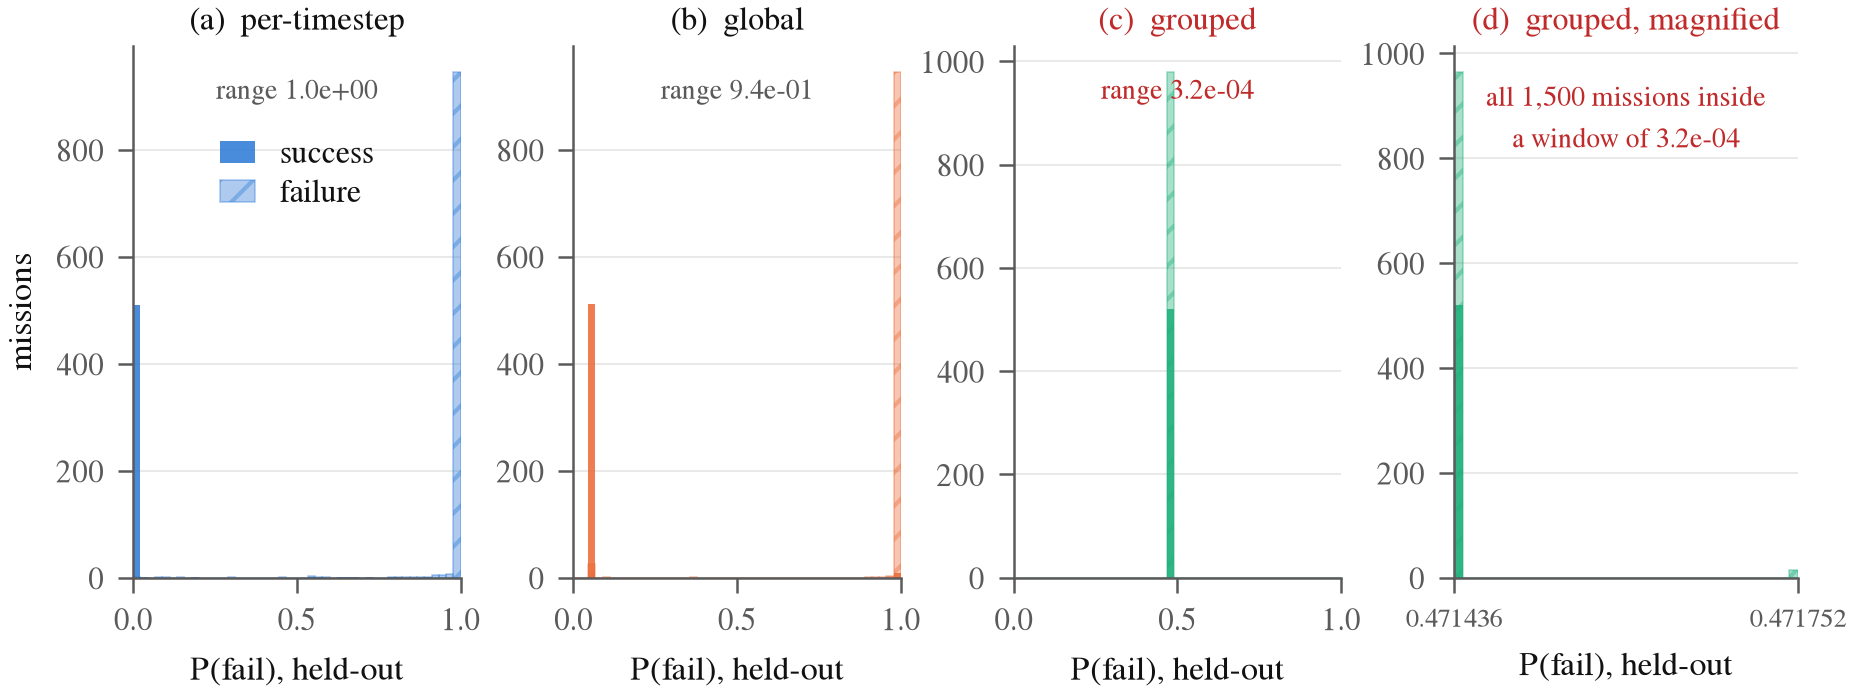
\includegraphics[width=\linewidth]{fig2.png}
\caption{P(fail) on Venus, split out for each setting. Per timestep and global normalisation put the two populations at opposite ends of the axis. Under grouped normalisation every mission gets essentially the same number. Panel (d) magnifies that spike and shows the full range covers about three ten-thousandths. This is what makes a collapse different from a merely bad model.}
\label{fig:venus}
\end{figure}

\begin{figure}[t]
\centering
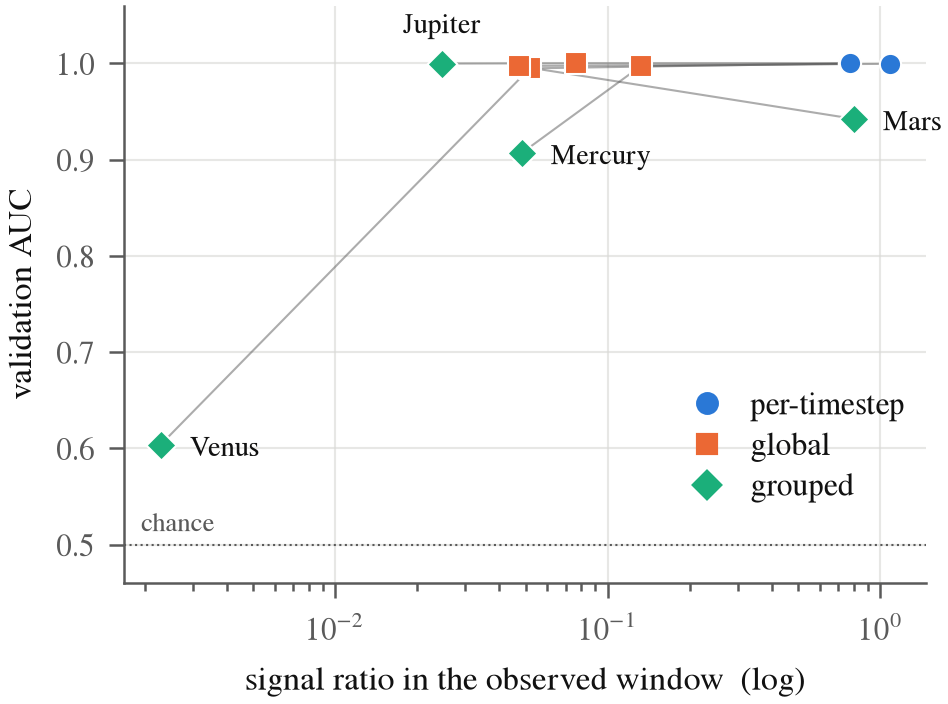
\includegraphics[width=\linewidth]{fig3.png}
\caption{Signal ratio against validation AUC. These points would lie on a curve if the collapse was only due to compression. Jupiter has a lower signal ratio than Mercury and still loses very little.}
\label{fig:signal}
\end{figure}

\begin{table}[t]
\centering
\caption{XGBoost on the same normalised window, for each setting. The tree is not affected by the preprocessing which destroys the network.}
\label{tab:xgb}
\begin{tabular}{@{}lcccc@{}}
\toprule
Target & per-timestep & global & grouped & spread \\
\midrule
Venus   & 1.0000 & 1.0000 & 1.0000 & 0.0000 \\
Mars    & 0.9996 & 0.9998 & 0.9998 & 0.0002 \\
Mercury & 0.9997 & 0.9998 & 0.9998 & 0.0001 \\
Jupiter & 1.0000 & 1.0000 & 1.0000 & 0.0000 \\
\bottomrule
\end{tabular}
\end{table}

\begin{figure}[t]
\centering
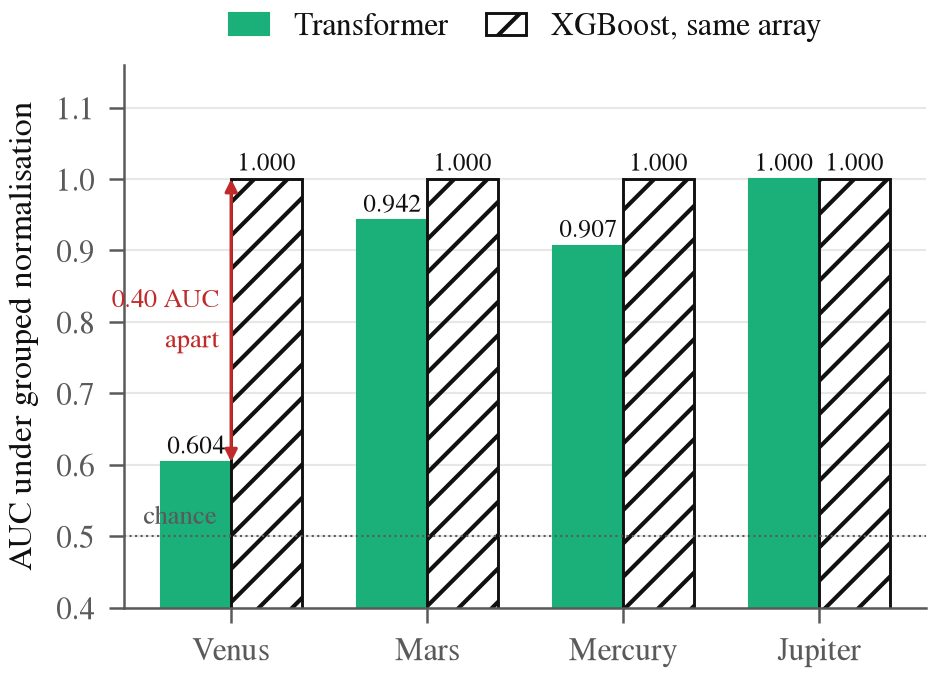
\includegraphics[width=\linewidth]{fig4.png}
\caption{Both models under grouped normalisation, on the same arrays. The tree is at the ceiling on every target, including the one where the network is just above chance.}
\label{fig:tree}
\end{figure}

\section{Does It Reproduce Across Seeds?}
\label{sec:seeds}

Is it spread by seed? All of the above is problematic in that it's one run deep. A bad initialisation could result in an AUC of only 0.6037. Thus, we redo the whole ablation in 5 different seeds, in each of which we redraw the train/validation/test partition and the initialisation.

Compression is not dependent on seed. The signal ratio for Venus under grouped normalisation lands between 0.00222 and 0.00232 across all 5 runs, a spread of 5\% against the compression of 335x itself. The healthy condition is stable too. The difference in per timestep AUC between two different seeds is at most 0.0010. There is no seed on which Mars, Mercury or Jupiter collapse.

It depends on the seed whether the network escapes or not. Venus collapses to a constant on 4 of 5 seeds, with prediction spread on unseen missions ranging from 1.57e-05 to 4.84e-05, which is 4 orders of magnitude lower than the 4.66e-01 obtained by correct normalisation. On the remaining seed it doesn't collapse, and it doesn't recover either: prediction spread 3.64e-02, still an order of magnitude short, at AUC 0.9305 against a healthy 0.9999. The preprocessing is then always sufficient for the collapse, but the collapse itself is not certain, only the usual outcome.

This is the real reason for the prediction spread diagnostic above. The range of grouped AUC for Venus over these runs is 0.5338 to 0.9305, which overlaps that of a merely weakened target. Mercury sits inside that range on every seed while still telling missions apart. AUC is thus unable to distinguish the two states. Prediction spread can. There are orders of magnitude between the collapsed runs and all the healthy runs. If you have to keep tabs on one number for this failure, watch that one.

The blindness of the baseline is repeated to a greater degree. Across 5 seeds, 4 targets and three normalisation settings, which is 60 fitted trees in total, the tree's AUC stays within the range 0.9989 to 1.0000, and within each seed and target the AUC difference is at most 0.0003 between settings. There is no seed on which the baseline notices. That matters more than the number of collapses. The collapse is one target's misfortune, but a check that can't fail is a property of the check.

\begin{table}[t]
\centering
\caption{Validation AUC across 5 seeds, mean and standard deviation, and the number of seeds on which the grouped run collapsed to a constant output.}
\label{tab:multiseed}
\begin{tabular}{@{}lccc@{}}
\toprule
Target & per-timestep AUC & grouped AUC & collapsed \\
\midrule
Venus   & $0.9998 \pm 0.0001$ & $0.6912 \pm 0.1530$ & 4/5 \\
Mars    & $0.9992 \pm 0.0004$ & $0.9457 \pm 0.0093$ & 0/5 \\
Mercury & $0.9997 \pm 0.0002$ & $0.9118 \pm 0.0036$ & 0/5 \\
Jupiter & $0.9999 \pm 0.0002$ & $0.9997 \pm 0.0003$ & 0/5 \\
\bottomrule
\end{tabular}
\end{table}

\begin{figure}[t]
\centering
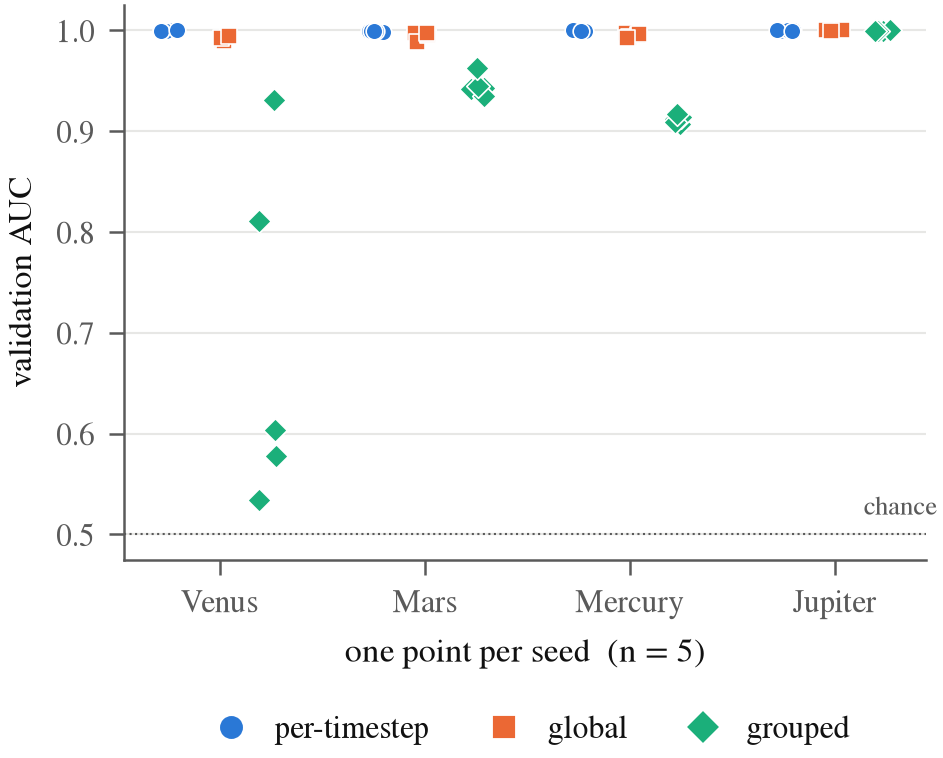
\includegraphics[width=\linewidth]{fig5.png}
\caption{Every seed plotted on its own rather than summarised as an interval. With n = 5 the spread of the raw points is the honest summary.}
\label{fig:seeds}
\end{figure}

\section{Failing to Reach a Signal That Is Present}
\label{sec:rare}

If the normalisation is correct, but the model doesn't pick up a signal that is there, the second failure appears. The failure mode \texttt{surface\_impact} makes up 91 of the 4,639 failures in training. A tree on the same normalised 40 step window separates that mode from success at AUC 1.0000, recall 1.0000. The recall of the sequence model at its operating point is 0.0000.

The information is there in both models and one of them splits the classes appropriately, so it is not an information limit, it's an optimisation limit in the sequence model. Resampling doesn't resolve the problem, which eliminates the most obvious explanation. We're not sure whether it is the loss landscape, or the CLS pooling discarding a cue that is localised in time, or the binary head being dominated by the majority mode. If we probe the representation of the trunk for linear separability of the rare mode it will narrow it down, and that's the next experiment, not a result we have.

This number can easily be quoted misleadingly, since it has two denominators. The rare mode is oversampled by about 45 times at the strongest setting, compared to the majority failure mode. The factor is 19.23x relative to uniform sampling over the training set, which is what the sampler actually applies. The latter is reported since it is what the optimiser saw.

The sweep was repeated on 5 seeds, which also redraw the split and therefore the rare mode itself. The gap replicates and the extremes do not. Sequence recall on the rare mode runs from 0.0000 to 0.1429 across all the seeds and sampling weights, against a tree on the same window at recall 0.9333 to 1.0000 and AUC 0.9997 to 1.0000. The sampling weight makes no difference on any one run at all: recall is the same at all three levels within a seed, so the flat line in the figure is not a property of a single run.

\begin{table}[t]
\centering
\caption{Oversampling sweep on the rare mode on Uranus. Turning up the sampling weight on the rare mode does not recover it, and does not disturb anything else either.}
\label{tab:oversample}
\begin{tabular}{@{}ccccc@{}}
\toprule
alpha & resample & test F1 & all modes & rare mode \\
\midrule
0.00 & 1.0x & 0.9938 & 0.9877 & 0.0000 \\
0.50 & 5.1x & 0.9938 & 0.9877 & 0.0000 \\
1.00 & 19.2x & 0.9938 & 0.9877 & 0.0000 \\
\bottomrule
\end{tabular}
\end{table}

\begin{figure}[t]
\centering
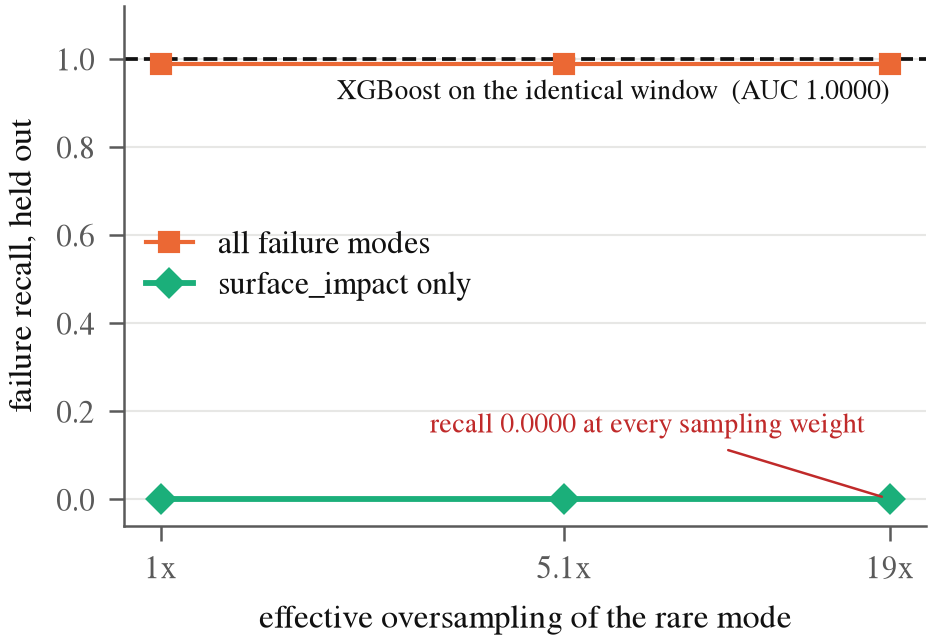
\includegraphics[width=\linewidth]{fig6.png}
\caption{Recall against oversampling weight. The horizontal line is a tree on the same window. The curve for the rare mode does not move.}
\label{fig:recall}
\end{figure}

\section{Where the Screen Belongs}
\label{sec:screen}

If it has been thoroughly done on the sequence model, the real answer is that it should not be used. The six feature classifier, which is evaluated prior to any propagation whatsoever, saves 64.5\% of compute against the telemetry model's 38.3\%, at a similar cost in good missions destroyed. There is also a levelling off of accuracy between 10\% and 40\% observed. The problem is not a modelling fault. The simulator is deterministic, the outcome is a fixed function of the injection offsets, and the trajectory is an integral of the offsets. It can't transport information that the parameters don't have.

This is not to imply that the task is trivial. Logistic regression on the same 6 features achieves 0.4824 to 0.5410 AUC on all of the targets, which is chance, so the mapping between the parameters and the outcome is very nonlinear and requires a learned model. A temporal one is not really necessary. The sequential screen is only worth applying if the outcome is not known at injection: mid flight stochasticity, unmodelled dynamics, sensor noise, or campaigns where the launch parameters are not known. That is exactly the setting reinforcement learning trajectory work needs when it certifies policies through dispersed Monte Carlo campaigns \citep{zavoli2021}.

This section is included since it sets the scope of the practical significance of all the preceding material. The methodological findings are valid for any grouped pipeline that models sequences. In the application that produced the findings, a sequence model was not needed at all. A reviewer who works that out alone is in a worse position than one who is told.

Two methodological remarks on this table, just before the conclusion we derive. The previous version was produced under two selection biases: the thresholds were optimised on the test labels, and the evaluation set contained the validation split of the sequence model. Both of them flattered T40, the screen that this section opposes. The headline moved by no more than 0.1 percentage points when they were removed. A negative result that survives its own correction is the strongest form the claim can take.

\begin{table}[t]
\centering
\caption{Screening economics. Compute is charged in propagation days, which span about a 100x range across the seven targets. Thresholds are fitted on validation and reported on the untouched test split, so the recall column is measured out of sample rather than achieved by construction.}
\label{tab:economics}
\footnotesize
\setlength{\tabcolsep}{4pt}
\begin{tabular}{@{}p{0.40\linewidth}ccc@{}}
\toprule
Screen & Compute saved & Good missions lost & Failure recall \\
\midrule
T0: six launch parameters, before propagating & 64.5\% & 0.76\% & 99.06\% \\
T40: telemetry Transformer at 40\% & 38.3\% & 0.21\% & 98.87\% \\
Cascade: T0 where confident, else T40 & 65.0\% & 1.62\% & 99.94\% \\
\bottomrule
\end{tabular}
\end{table}

\begin{figure}[t]
\centering
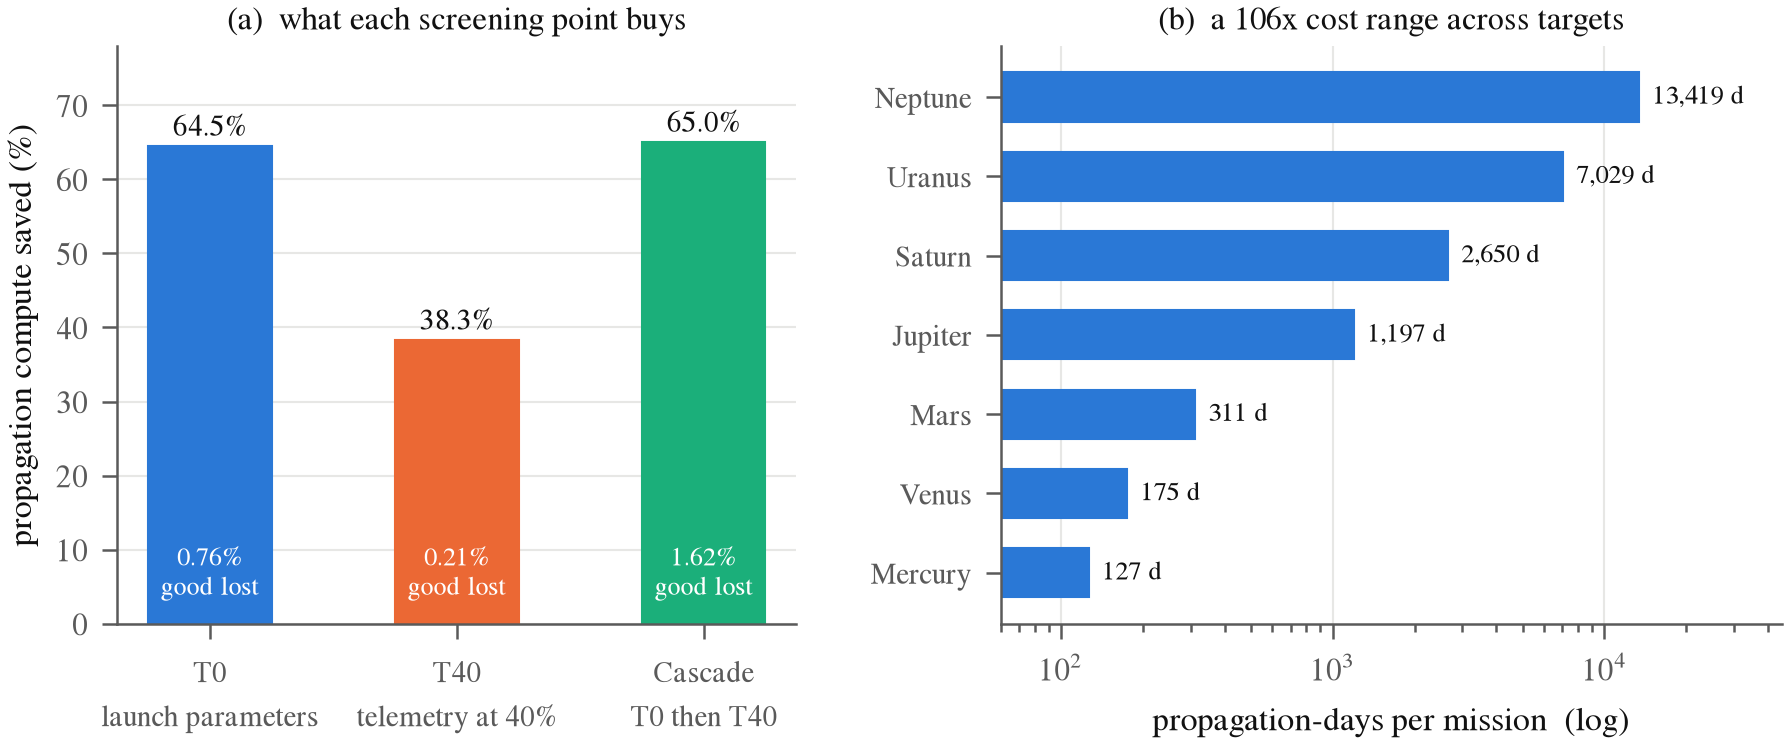
\includegraphics[width=\linewidth]{fig7.png}
\caption{(a) What each screening point buys and what it costs. (b) Why the weighting is not uniform: the cost of propagating one mission spans two orders of magnitude, so the value of a screen is dominated by the outer targets.}
\label{fig:economics}
\end{figure}

\section{Limitations}
\label{sec:limitations}

\begin{itemize}
\item Seeds. Replication: 5 seeds. This is enough to exclude an unfortunate initialisation, but not to warrant a narrow confidence interval. We report the spread of the individual runs and not a fitted interval. The collapse itself comes at 4/5, and the exception is likely subject to a controlling factor, but that just isn't known with a small sample.
\item One corpus. The collapse is shown on one data set. We outline the mechanism in terms of a variance ratio which is not specific to astrodynamics, but we have not reproduced it on a second data set and any threshold on this ratio that makes a claim to predicting the collapse is therefore a guess, rather than a discovery.
\item Four targets in the ablation. 1 of 4 targets collapses. All four agree on the result concerning the blind baseline, which is the half concerning method.
\item Synthetic and deterministic. There are no execution errors, no unmodelled accelerations, no sensor noise and all missions of a target have a common time base. This common time base is what makes standardisation per timestep possible at all and it is not a property of a real campaign, but of the generator.
\item No real mission data. This is the most serious issue of external validity. There are now available real satellite telemetry public benchmarks \citep{kotowski2024,hundman2018} and they are the natural next benchmarks for the diagnostic.
\end{itemize}

\section{Conclusion}
\label{sec:conclusion}

In the case that a feature scaler is used in multiple groups, where each group has their own scale, then a deep model can become into a per group constant, and a tree on the same arrays will return that the solution has been found. None of the pieces here are exotic. One of the default decisions of a standard pipeline is the preprocessing. The model used is just a plain Transformer. The usual one, that the people would pick up is the baseline. The standard defence, the checking of a simple baseline, is constructed so as not to be able to see the defect, which makes it impossible to fail the broken model.

We don't claim the fix, normalisation per group, to be new. The problem to be solved is the detection problem: there is a check which is executed regularly and which certifies a broken configuration, and then another check which is not expensive, but which catches the broken configuration. If the range of the predictions in each group had been given in addition to the summary numbers, we would have spotted ours quickly.

\section{Code and Data Availability}
\label{sec:code}

All the scripts for the experiments, the JSON artifacts that each number is read from, the code for the figures and the source of this document are available in a public repository (URL withheld for double-anonymized review). A short map of where things are:

\begin{sloppypar}
\texttt{src/ml/} holds the experiments. \texttt{norm\_ablation.py} produces Table~\ref{tab:ablation}, \texttt{baseline\_invariance.py} Table~\ref{tab:xgb}, \texttt{rare\_mode\_sweep.py} Table~\ref{tab:oversample} and \texttt{prune\_economics.py} Table~\ref{tab:economics}. All of them share the same definition of the train/validation/test partition, in \texttt{splits.py}.
\end{sloppypar}

\texttt{src/ml/model.py} is the Transformer, and \texttt{planet\_config.py} holds the target list, the cadences and the recorded reason the Moon is excluded.

\texttt{reports/} holds the measured artifacts. Every table and figure in this document comes from one of those JSON files, and \texttt{multiseed\_paper/} holds the runs at each seed behind Table~\ref{tab:multiseed}.

\texttt{docs/RESEARCH\_LEDGER.md} is the complete decision history, including two analyses that were invalidated by a positional join and the corrections that replaced them. \texttt{docs/LIMITATIONS.md} states what the results do not support.

The JSON creates the tables and figures in this manuscript and not the other way round. No number was typed into the manuscript by hand.

The experiments read per target \texttt{.npz} files of roughly 70 MB each, which are derived from a 71 GB mission table that is too large to store in the repository. The scripts below regenerate the artifacts from those extracts. \texttt{ORBITGUARD\_DATA} points at the full table, and the economics analysis is the only experiment that needs it.

{\scriptsize
\begin{verbatim}
export ORBITGUARD_DATA=/path/to/dataset

# Primary results, seed 42
python -m src.ml.norm_ablation          # Table 1
python -m src.ml.baseline_invariance    # Table 2
python -m src.ml.rare_mode_sweep        # Table 4
python -m src.ml.prune_economics        # Table 5

# Replication, one pass per seed (Table 3, Section 5)
for S in 0 1 2 3; do
  python -m src.ml.norm_ablation --seed $S \
      --out reports/multiseed_paper/normalisation_ablation_seed$S.json
  python -m src.ml.baseline_invariance --seed $S \
      --out reports/multiseed_paper/baseline_invariance_seed$S.json
  python -m src.ml.rare_mode_sweep --seed $S \
      --out reports/multiseed_paper/rare_mode_sweep_seed$S.json
done

# The document
python docs/paper/build/collect_traces.py   # Fig. 2 data
python docs/paper/build/figures.py          # all figures
python docs/paper/build/render_latex.py     # this document
\end{verbatim}
}

%% Competing interest, CRediT, and funding are on title_page.tex.

\section*{Declaration of Generative AI and AI-assisted technologies in the writing process}
During the preparation of this work the authors used Claude (Anthropic) in order to write and debug code, draft parts of the text, and check references. After using this tool, the authors reviewed and edited the content as needed and take full responsibility for the content of the publication.

\bibliographystyle{elsarticle-harv}
\bibliography{references}

\end{document}
